\documentclass[aspectratio=43]{beamer}
\mode<presentation>
\usetheme{Madrid}
\usecolortheme{seahorse}
% \usepackage[table]{xcolor}
\usepackage{multimedia}
\usepackage{media9}
\usepackage[utf8]{inputenc}
\usepackage{amsmath}
\usepackage{lmodern}
% \usepackage[usenames, dvipsnames]{color}

\usepackage{arydshln}
\usepackage{url}
\usepackage[absolute,overlay]{textpos}
\setlength{\TPHorizModule}{\textwidth}
\setlength{\TPVertModule}{\textwidth}

\graphicspath{{../../../Papers/The300/plots/}}

\setbeamercolor{CBwonb}{fg=white,bg=white!10!blue}
\setbeamercolor{CBronb}{fg=red,bg=white!10!blue}

\usepackage{tikz}
\usetikzlibrary{shapes,arrows,positioning}
\tikzstyle{startstop} = [rectangle, rounded corners, minimum width=1cm, minimum height=0.1cm,text centered, text width=2.5cm, draw=black, fill=red!30]
\tikzstyle{io} = [trapezium, trapezium left angle=70, trapezium right angle=110, minimum width=1cm, minimum height=0.1cm, text centered, text width=2.5cm, draw=black, fill=blue!30]
\tikzstyle{process} = [rectangle, minimum width=1cm, minimum height=0.1cm, text centered,text width=2.5cm, draw=black, fill=orange!30]
\tikzstyle{decision} = [circle, minimum width=1cm, minimum height=0.1cm, text centered,text width=2.5cm, draw=black, fill=green!30]
\tikzstyle{arrow} = [thick,->,text centered, color=blue, text width=2cm,>=stealth]

\newcommand{\Msun}{~{\rm M_\sun}}
\newcommand{\hMsun}{~h^{-1}\>{\rm M_\odot}}
\newcommand{\Mpc}{~h^{-1}~{\rm Mpc}}
\newcommand{\Kpc}{~h^{-1}~{\rm kpc}}


\title[]{The Three Hundred}
\subtitle{A short overview}
\author[Email: weiguang.cui@uam.es]{{\Large \bf Weiguang Cui},\inst{*} \footnote{\url{https://weiguangcui.github.io}}\\
In collaboration with the core team and players.}
\institute[]{
  \inst{*}
  Departamento de F\'isica Te\'{o}rica, \\
  Universidad Aut\'{o}noma de Madrid, 28049 Madrid, Spain
}
\date[]{Newbattle Abbey, Edingburgh, June 4, 2018}
\logo{
\includegraphics[height=1cm]{./plots/logo_uam.jpg}}

%%%%%%%%%%%%%%%%%%%%%%%%%%%%%%%%%%%%%%%%%%%%%%%%%%%%%%%%%%%%%%%%%%%%%%%%%
\begin{document}
  \frame{\titlepage}

%----------------------------------
\section{Introduction} \label{sec:1}

% \begin{frame}
%   \frametitle{Background: Cluster of Galaxies:}
%     \begin{itemize}
%       \item<1-> Galaxy cluster is the final state of the hierarchical structure formation.
%       \item<2-> Typically a few Mpc across, contain $\sim$ 100 - 1000 luminous galaxies and many more dwarfs, masses $\gtrsim 10^{14.5} M_{\odot}$.
%       \item<3-> Dark matter: $\sim 85 \%$, gas: $\sim 13 \%$, star: $\sim 1 - 2 \%$.
%       \item<4-> It provides plentiful information for baryonic processes, galaxy formation and cosmology models.
%       \item<5->[]
%         \begin{figure}
%           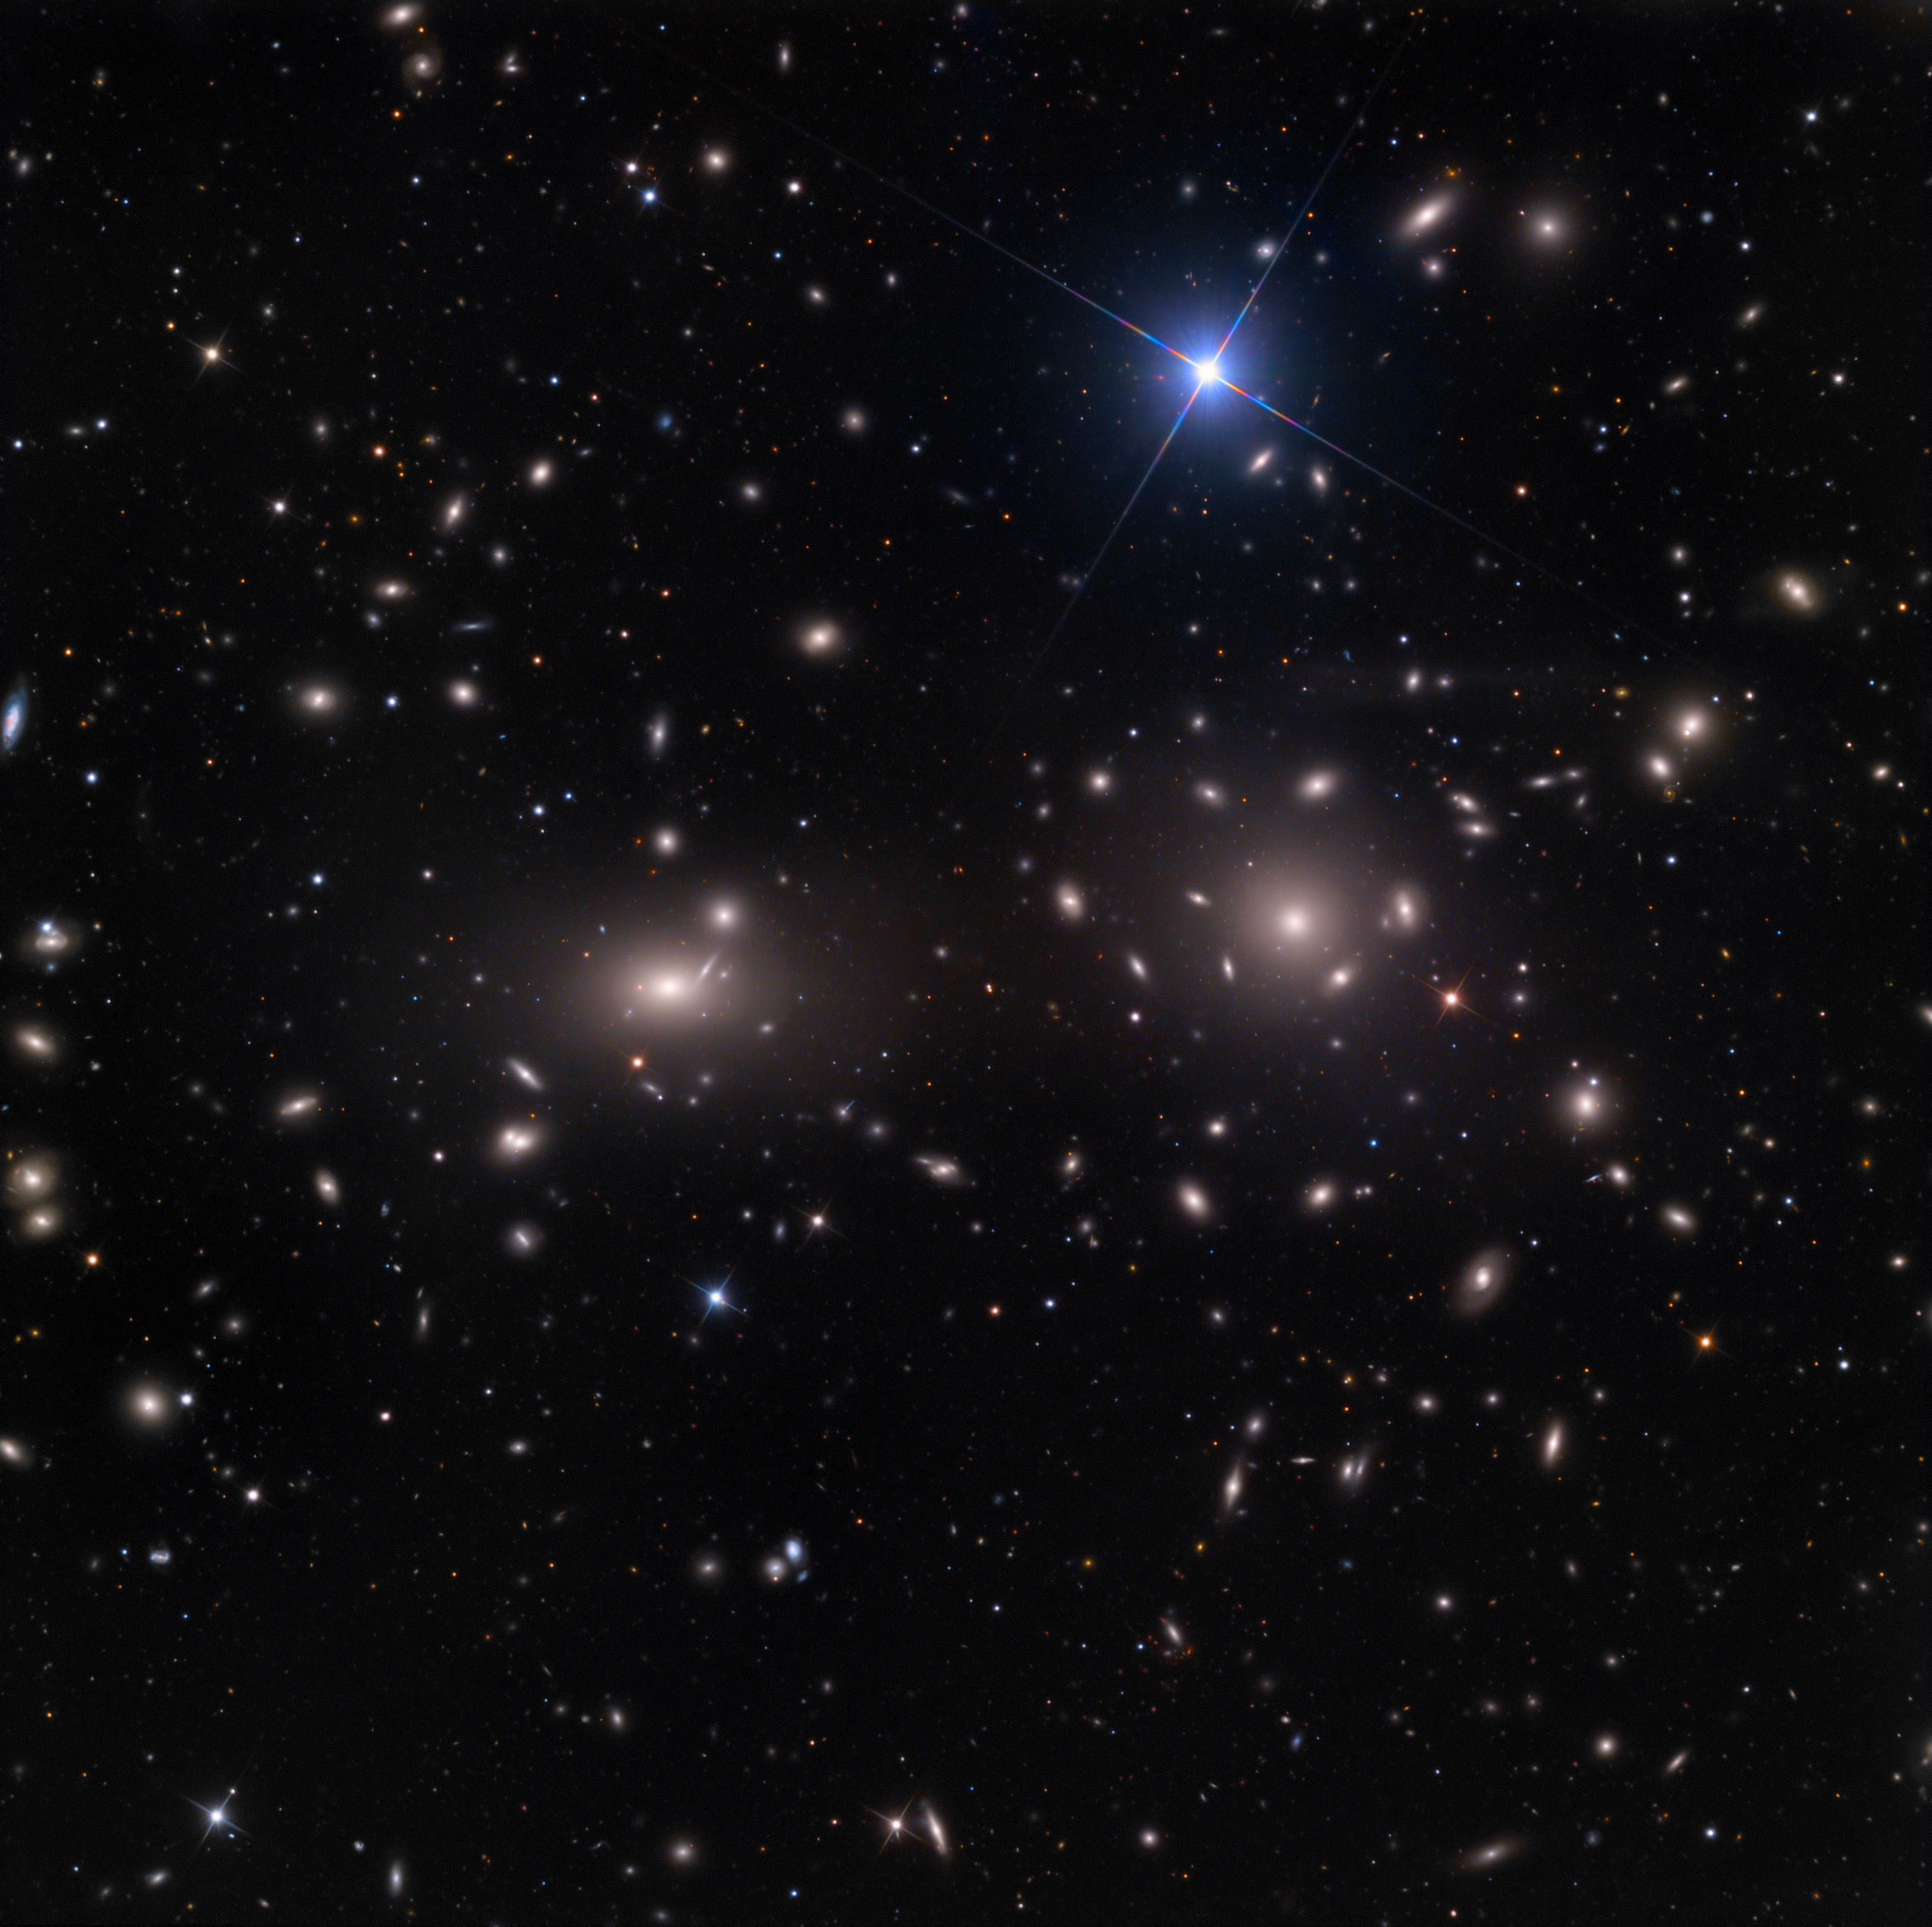
\includegraphics[width=0.292\textwidth]{Coma-SDSS.jpg}
%           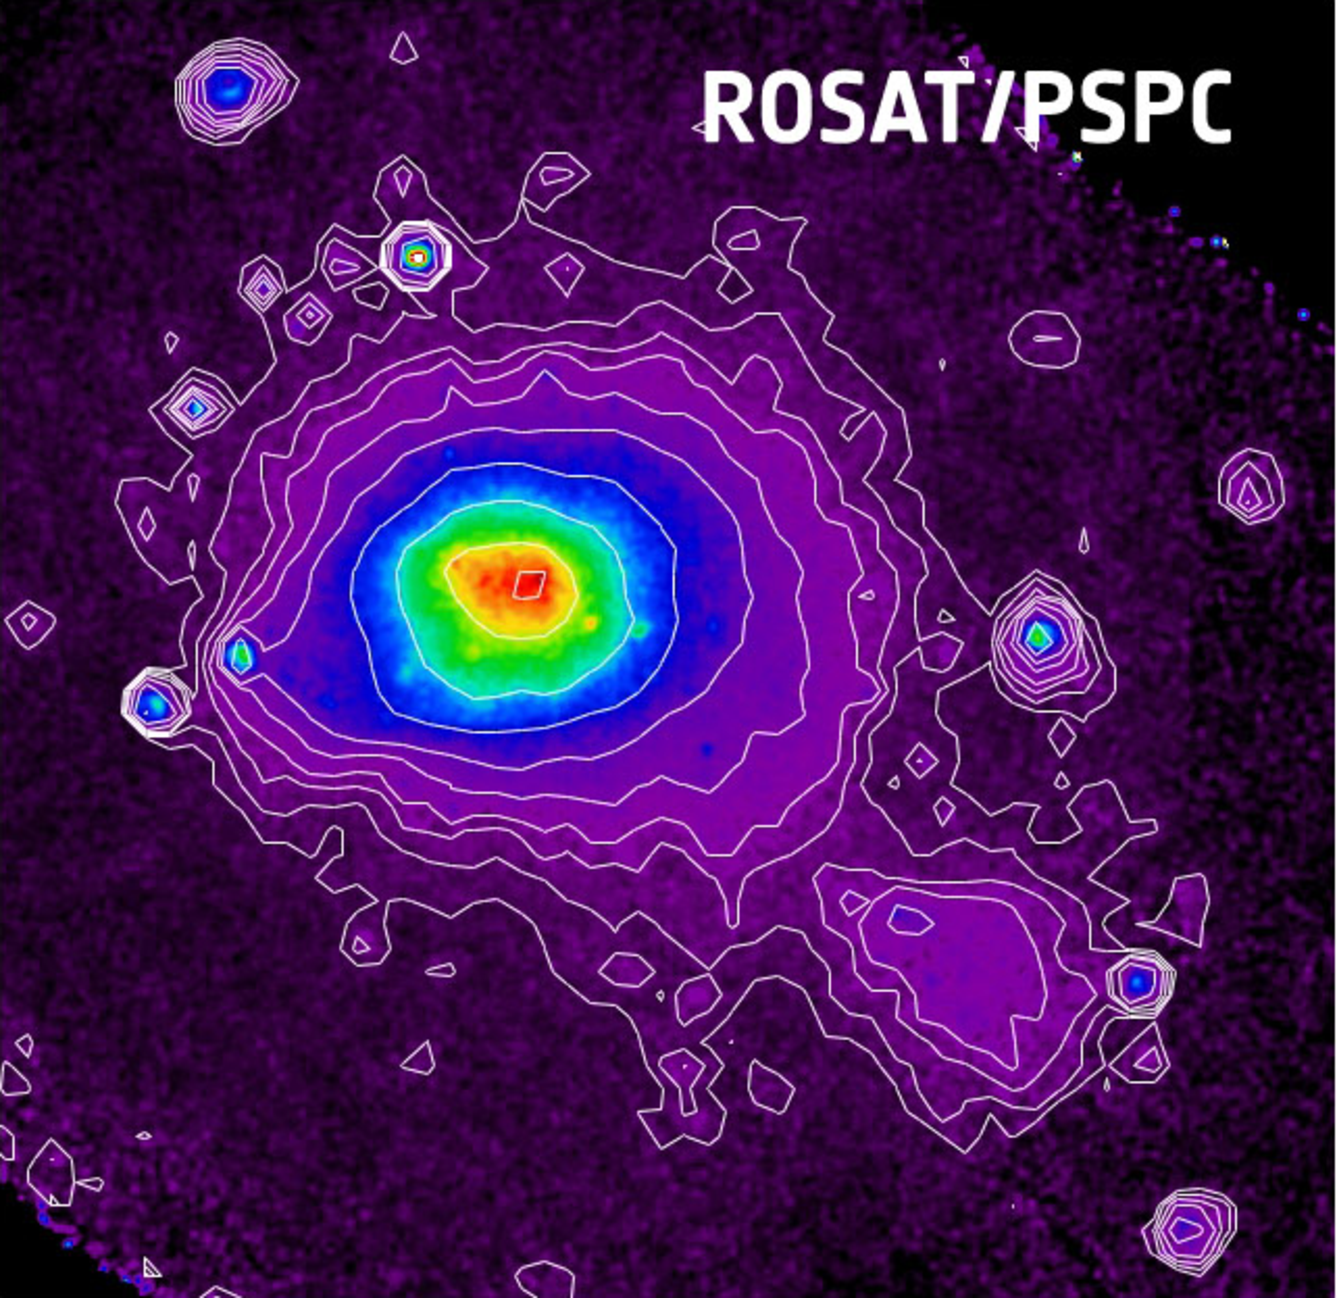
\includegraphics[width=0.3\textwidth]{Coma-Rosat.pdf}
%           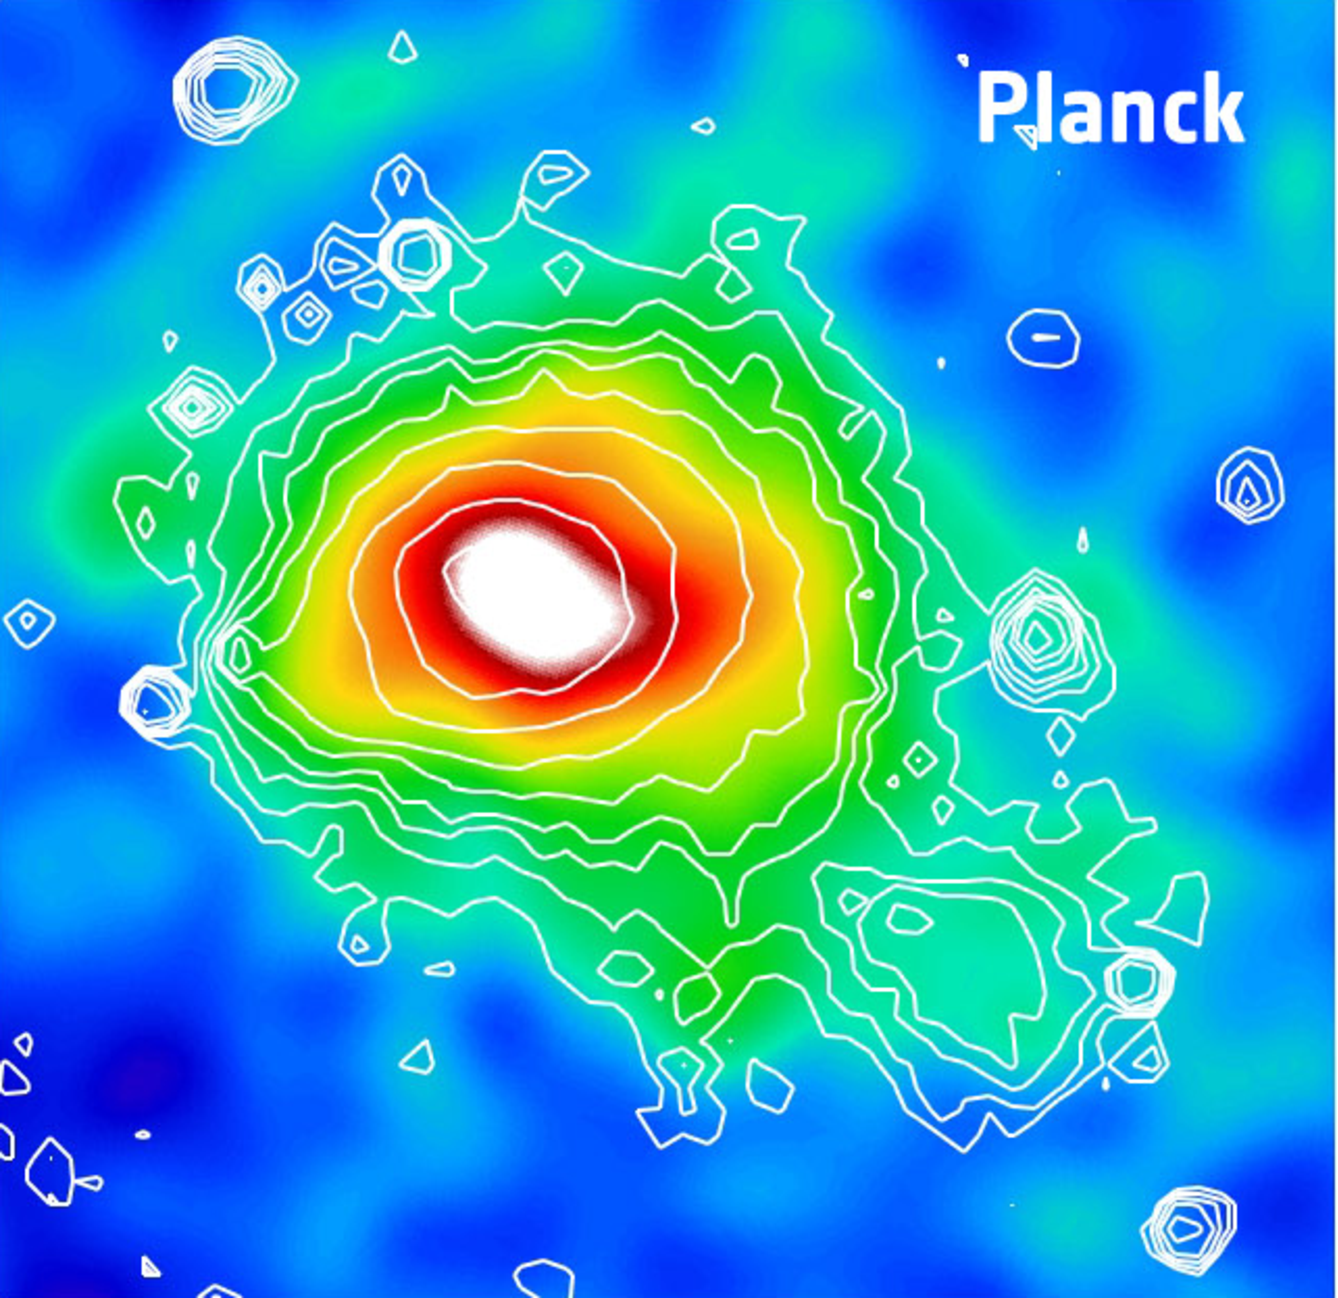
\includegraphics[width=0.3\textwidth]{Coma-Planck.pdf}
%           \vspace{-0.4cm}
%           \caption{The Coma cluster.}
%         \end{figure}
%     \end{itemize}
% \end{frame}
%
% \begin{frame}
%   \frametitle{Background: Cluster of Galaxies:}
%   {\bf To understand these observational results, especially how they are formed, we need simulations.}
%
%   \begin{center}
%     \movie[loop,autostart]{\includegraphics[width=0.4\textwidth]{G3X-17-image.pdf}}{plots/NewMDCLUSTER_0017.mp4}
%   \end{center}
%   % \begin{textblock}{0.25}(0.05,0.4)
%   %   {\scriptsize Cluster 17 \\ credit: Gustavo Yepes.}
%   % \end{textblock}
% \end{frame}
%
% \begin{frame}
%   \frametitle{The Three Hundred: A successor of the {\sc nIFTy} project}
%   \only<1>{
%     \begin{center}
%       {\Large \bf The {\sc nIFTy} galaxy cluster comparison project}\footnote{\scriptsize Ref: Sembolini et al. 2016a,b; Elahi et al. 2016; Cui et al. 2016; Arthur et al. 2017}
%     \end{center}
%     \alert{11} different (in both algorithms and baryon models) simulation codes are used to simulate the same galaxy cluster.
%     \begin{figure}
%       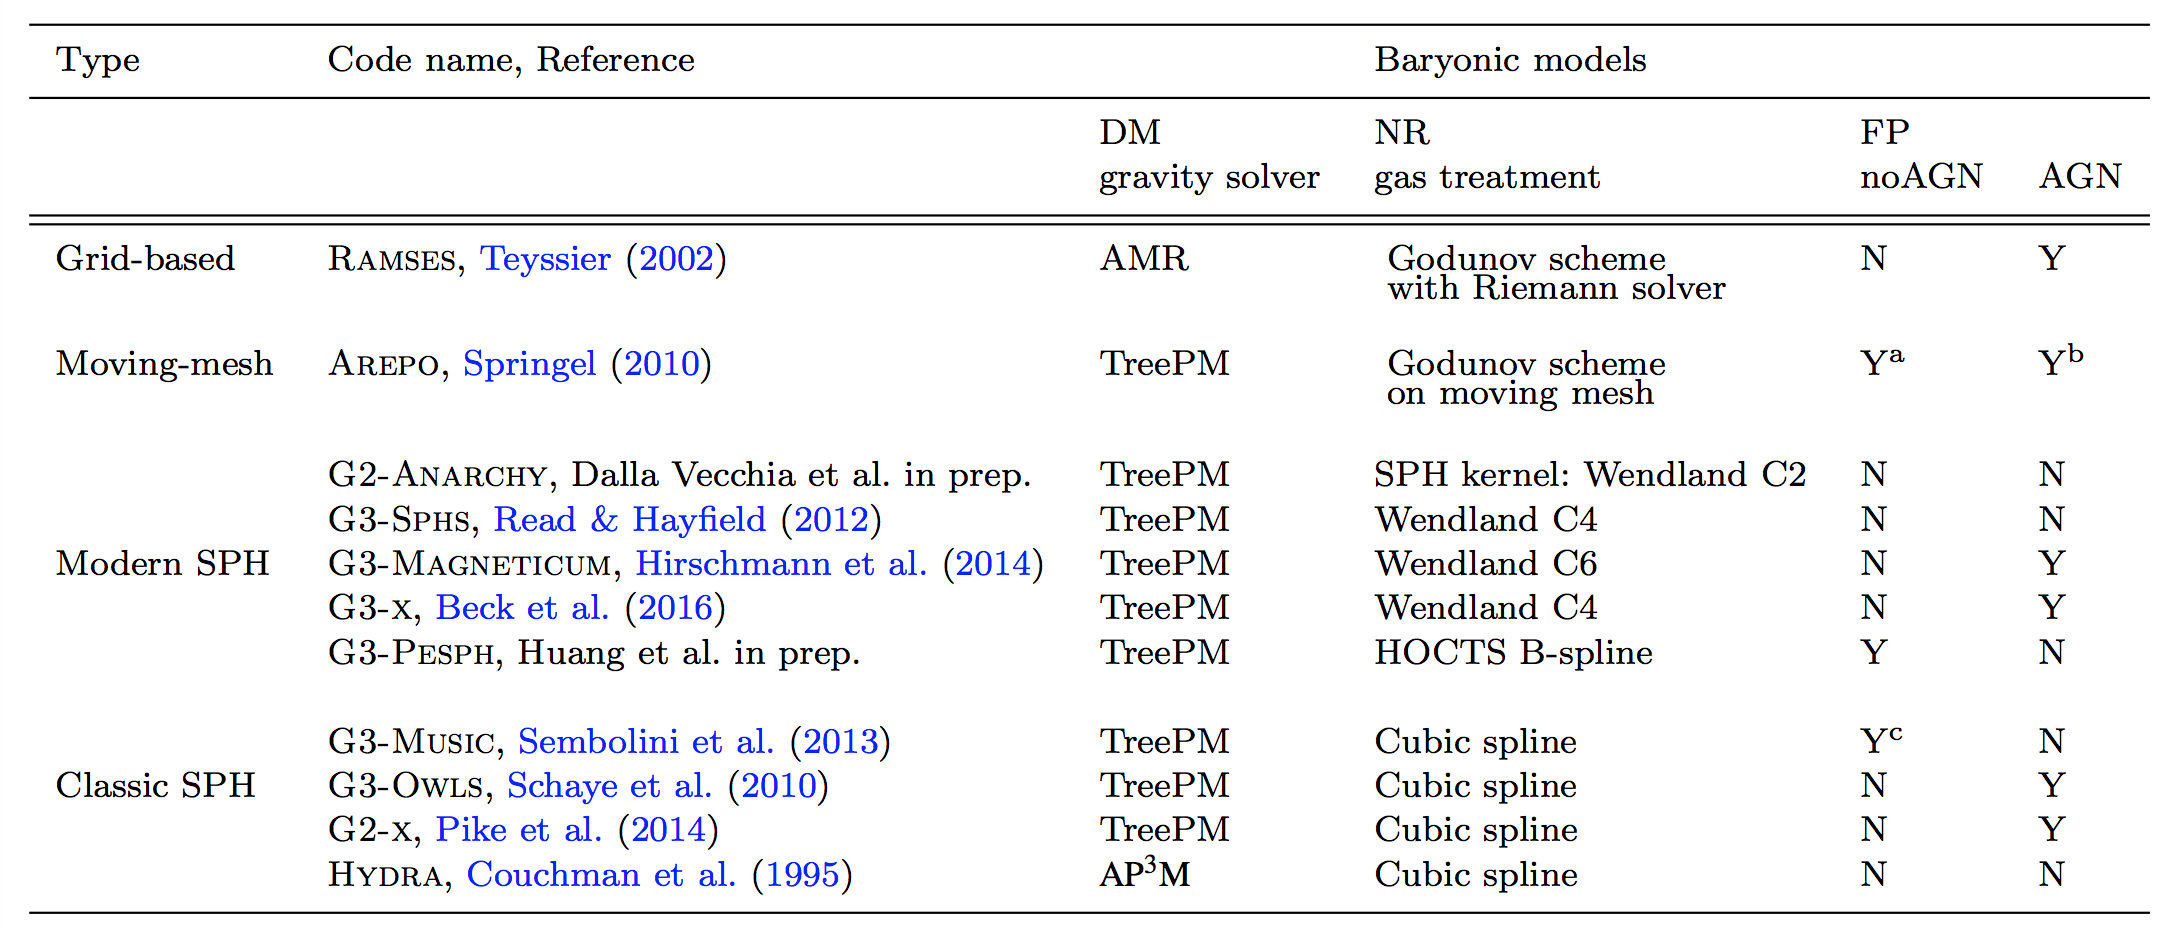
\includegraphics[width=0.9\textwidth]{nifty-codes.png}
%       % \caption{{\small Sembolini et al. 2016a, 2016b.}}
%     \end{figure}
%   }
%   \only<2>{
%     \begin{center}
%       {\Large \bf What did we find? I}
%     \end{center}
%     {\scriptsize
%     \begin{itemize}
%       \item The modern SPH codes produce correct entropy profiles as AMR, moving mesh.
%       \item The baryon models have larger effects than the fluid simulating techniques by mixing the entropy profiles.
%     \end{itemize}}
%     \begin{figure}
%       \vspace{-0.2cm}
%       \includegraphics<2>[width=0.36\textwidth]{nifty-entropy.png}
%       \includegraphics<2>[width=0.45\textwidth]{nifty-entropy-fp.png}\vspace{-0.4cm}
%       % \caption{{\scriptsize Entropy profile. Ref: Sembolini et al. 2016a,b}}
%     \end{figure}
%     \begin{textblock}{0.12}(0.01,0.3)
%       {\scriptsize  Entropy profile. \\ Ref: Sembolini et al. 2016a,b.}
%     \end{textblock}
%   }
%   \only<3>{
%     \begin{center}
%       {\Large \bf What did we find? II}
%     \end{center}
%     {\scriptsize
%     \begin{itemize}
%       \item Different baryon models produce similar global properties, large scatter at small scales.
%     \end{itemize}}
%     \begin{figure}
%       \includegraphics<3>[width=0.4\textwidth]{be-dp}
%       % \includegraphics<2>[width=0.45\textwidth]{nifty-entropy-fp.png}
%     \end{figure}
%     \begin{textblock}{0.25}(0.05,0.4)
%       {\scriptsize E.g. Baryon effects on density profile. \\ Ref: Cui et al. 2016}
%     \end{textblock}
%     }
%   \only<4>{
%     \begin{center}
%       {\Large \bf What's next?}
%     \end{center}
%     \alert{Aim: } to understand the formation and evolution of galaxy clusters.
%     \begin{itemize}
%       \item Comparisons between models to understand the theoretical predictions.
%       \item Comparisons between models and observations to constrain the models.
%     \end{itemize}
%
%   ~
%
%   \alert{\Large A large cluster sample!}
%   }
%   % \begin{enumerate}
%   %   \item \alert{Code} My own SSP code -- pymgal (inherited from EzGal)
%   %   \item \alert{Location} \path{~/TheThreeHundred/maps/CCD/<simulation code name>/NewMDCLUSTER_XXXX/}
%   %   \item \alert{Notes}
%   %   \begin{itemize}
%   %     \item 1) 5 SDSS + 3 HST filters are provided. Mass + age + metal in
%   %   \end{itemize}
%   % \end{enumerate}
% \end{frame}

\section{The Three Hundred}
\begin{frame}
  \frametitle{The Three Hundred: Basic information}
  \begin{itemize}
    \item The most massive ($M_{vir} > 8\times 10^{14} \hMsun$) 324 clusters are selected from the MultiDark simulation(MDPL2)\footnote{\url{https://www.cosmosim.org}}.
    \item 324 zoomed-in ICs are generated by cutting a spherical region with a radius of \alert{$15 \Mpc$} from the cluster center.
    \item[]
      \begin{table}
        \fontsize{10}{10}\selectfont
        \caption{Parameters of the Three Hundred simulations}
        \begin{tabular}{lll}
          \hline
          Parameter& Value & Description\\
          \hline
          $\Omega_M$ & 0.307 & Total Matter density parameter\\
          $\Omega_B$ & 0.048 & Baryon density parameter\\
          $\Omega_\Lambda$ & 0.693 & Cosmological Constant density parameter\\
          $h$ & 0.678  & Hubble constant in units of 100 km/s/Mpc\\
          $\sigma_8$ & 0.823 & Normalization of Power spectrum\\
          $n_s$ & 0.96  & Power index\\
          % $f_B$ & 0.0696&  Cosmic Baryon Fraction\\
          $z_{init}$ & 120 & Initial redshift of the simulations \\
          $\epsilon_{phys}$ & 6.5 & Plummer equivalent softening in $\Kpc$ \\
          % Box size & 1 $h^{-1} Gpc$ (15 $\Mpc$) & The MDPL2 simulation box on one side (the radius for each re-simulation region) \\
          Particle mass & $2.36 \ (12.7) $ & gas (DM) in [$10^8 \hMsun$]\\
          \hline
        \end{tabular}
      \end{table}
\end{itemize}
% \vspace{-0.6cm}
\end{frame}

\begin{frame}
  \frametitle{The Three Hundred: theoretical models}
  \begin{columns}[t]
    \begin{column}{0.55\textwidth}
      \begin{block}{hydrodynamical simulations with baryonic models:}
        {\sc Gadget-\alert{MUSIC}}: classic SPH method. Radiative cooling, star formation with both thermal and kinetic Supernove (SN) feedback.

        {\sc Gadget-\alert{X}}: modern SPH with the Wendland C4 kernel. Gas cooling with metal contributions, star formation with chemical enrichment, SN feedback with AGB phase, and AGN feedback.

        {\sc GIZMO-\alert{Mufasa/Simba}:} see more information in Mika/Romeel's talks.

        {\sc Gadget-\alert{PESPH:}} running.
      \end{block}
    \end{column}
    \begin{column}{0.42\textwidth}
      \begin{block}{SAMs galaxies from MultiDark-Galaxies:}
        {\sc Galacticus}

        {\sc SAG} see more information in Sofia's talk.

        {\sc SAGE}. see more information in Adam's talk.

        See Knebe et al. 2018 (MNRAS, 474, 5206), for details.

        Notes: only galaxies/clusters from \alert{the same regions} as the hydrodynamical simulations are selected.
      \end{block}
    \end{column}
  \end{columns}
  % A coupling with MultiDark-Galaxies
\end{frame}

\begin{frame}
  \frametitle{The Three Hundred: what do we have for playing?}
  \begin{table}
    \fontsize{6}{6}\selectfont
    % \caption{Parameters of the Three Hundred simulations}
    \begin{tabular}{llllllllll}
      \hline
      Simulations & snaps & AHF & Rocks. &VELOCIr. & dynamic & CCD & SZ & XRAYS & lensing\\
      \hline
      MDPL2 & \textcolor{green}{324 regions} & \textcolor{green}{done} & \textcolor{green}{done} & \textcolor{yellow}{?} & \textcolor{blue}{z=0} & \textcolor{red}{X} & \textcolor{red}{X} & \textcolor{red}{X} & \textcolor{yellow}{?} \\
      &\textcolor{blue}{4 outputs}&&&&&&&&\\
      \hdashline
      GadgetX & 324 regions & \textcolor{green}{done} & \textcolor{yellow}{?} & \textcolor{yellow}{?} & \textcolor{blue}{4 snaps} & \textcolor{blue}{few} & \textcolor{blue}{z=0} & \textcolor{blue}{z=0} & \textcolor{yellow}{?}\\
      &\textcolor{green}{128 outputs}&&&&&&&&\\
      MUSIC & 324 regions& \textcolor{green}{done} & \textcolor{yellow}{?} & \textcolor{yellow}{?} & \textcolor{blue}{4 snaps} & \textcolor{blue}{few} & \textcolor{blue}{z=0} & \textcolor{blue}{z=0} & \textcolor{yellow}{?}\\
      &\textcolor{blue}{17/128 outputs}&&&&&&&&\\
      MUFASA & few regions & \textcolor{green}{done} & \textcolor{yellow}{?} & \textcolor{yellow}{?} & \textcolor{yellow}{?} & \textcolor{yellow}{?} & \textcolor{yellow}{?} & \textcolor{yellow}{?} & \textcolor{yellow}{?}\\
      &\textcolor{green}{128 outputs}&&&&&&&&\\
      Simba & few regions& \textcolor{green}{done} & \textcolor{yellow}{?} & \textcolor{yellow}{?} & \textcolor{yellow}{?} & \textcolor{yellow}{?} & \textcolor{yellow}{?} & \textcolor{yellow}{?} & \textcolor{yellow}{?}\\
      &\textcolor{green}{128 outputs}&&&&&&&&\\
      PESPH & \textcolor{yellow}{?} & \textcolor{yellow}{?} & \textcolor{yellow}{?} & \textcolor{yellow}{?} & \textcolor{yellow}{?} & \textcolor{yellow}{?} & \textcolor{yellow}{?} & \textcolor{yellow}{?} & \textcolor{yellow}{?}\\
      &\textcolor{yellow}{?}&&&&&&&&\\
      \hdashline
      SAMs &&&&&&&&&\\
      Galacticus& \textcolor{green}{324 regions} & \textcolor{red}{X} & \textcolor{red}{X} & \textcolor{red}{X} & \textcolor{red}{X} & \textcolor{red}{X} & \textcolor{red}{X} & \textcolor{red}{X} & \textcolor{red}{X}\\
      &\textcolor{blue}{z=0 outputs}&&&&&&&&\\
      SAG & \textcolor{green}{324 regions} & \textcolor{red}{X} & \textcolor{red}{X} & \textcolor{red}{X} & \textcolor{red}{X} & \textcolor{red}{X} & \textcolor{red}{X} & \textcolor{red}{X} & \textcolor{red}{X}\\
      &\textcolor{blue}{z=0 outputs}&&&&&&&&\\
      SAGE & \textcolor{green}{324 regions} & \textcolor{red}{X} & \textcolor{red}{X} & \textcolor{red}{X} & \textcolor{red}{X} & \textcolor{red}{X} & \textcolor{red}{X} & \textcolor{red}{X} & \textcolor{red}{X}\\
      &\textcolor{blue}{z=0 outputs}&&&&&&&&\\
      \hline
    \end{tabular}
  \end{table}
\end{frame}

\begin{frame}
  \frametitle{The Three Hundred: the catalogues}
    Halos and subhalos in hydrodynamical simulations are identified with AHF (Ref: Knollmann \& Knebe 2009).
    % The luminosity/magnitude of the galaxies are calculated with STARDUST (Ref: Deriendt et al. 1999).
    \only<1>{
    \begin{figure}
      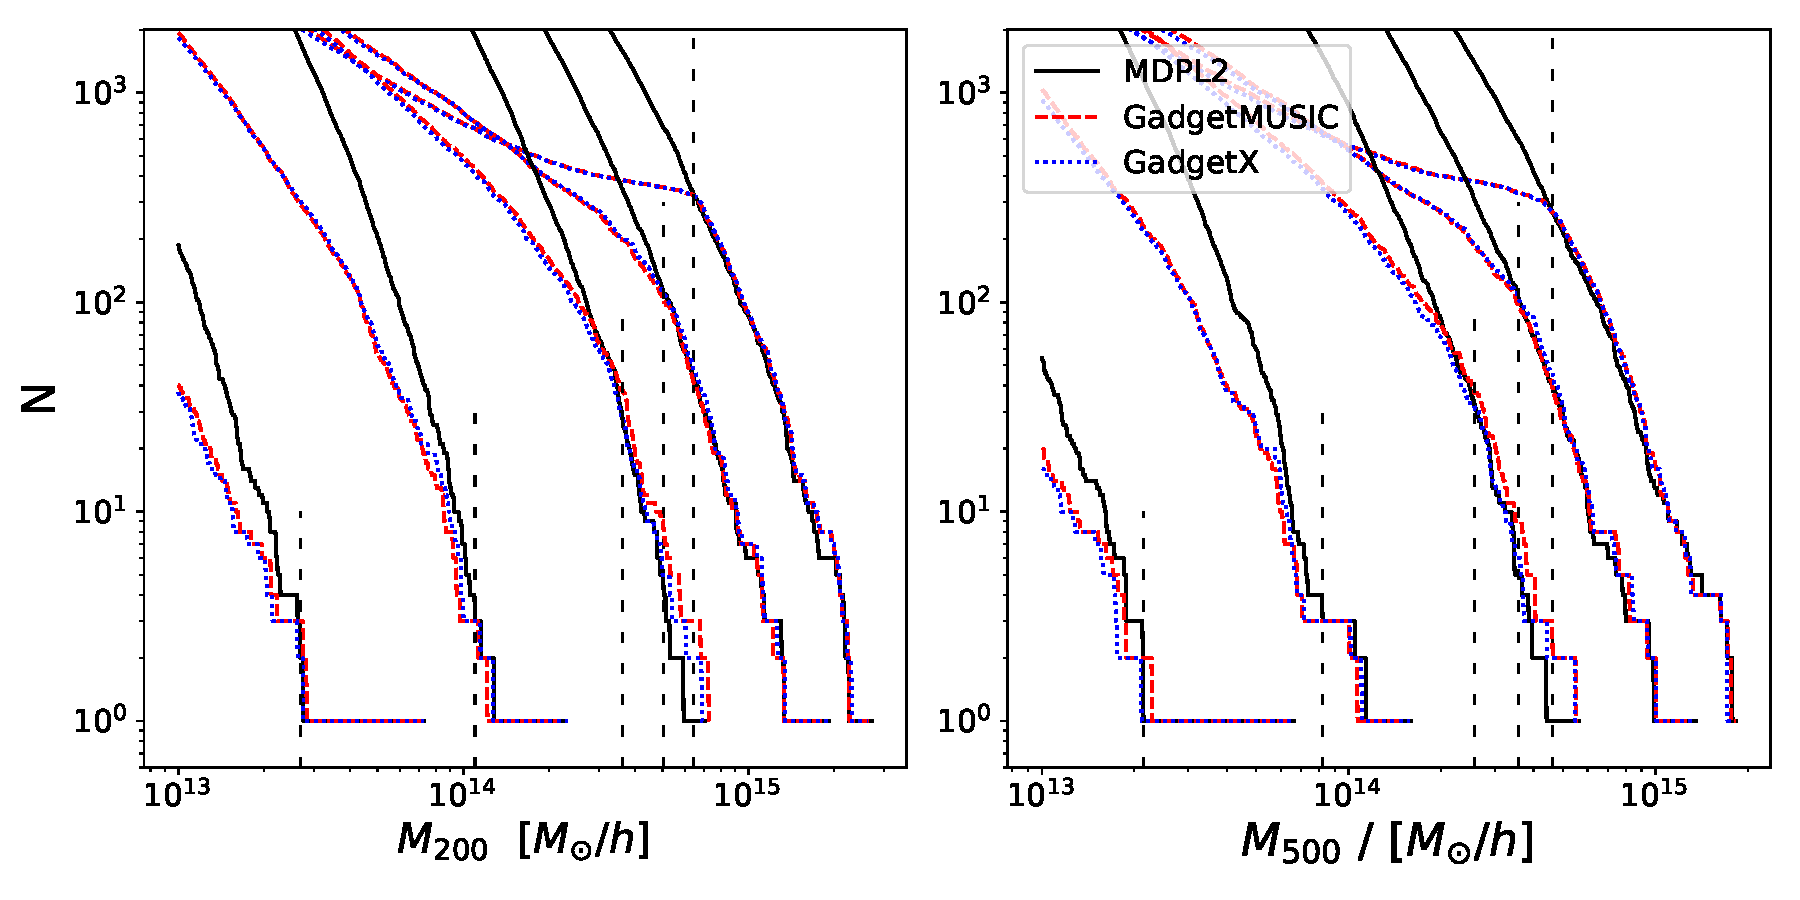
\includegraphics[width=0.9\textwidth]{HMF_full.pdf}
      \vspace{-0.6cm}
      \caption{Cumulative halo mass functions. }
    \end{figure}}
    \only<2>{
      \begin{table}
    	\centering
    	\caption{The \alert{infamous complete} sample of the Three Hundred cluster catalogues at different redshifts.}
    	\label{tab:masscomplete}
    	\begin{tabular}{lcccc} % four columns, alignment for each
    		\hline
    		redshift & $M_{200c}$  & $N_{200c}$ & $M_{500c}$  & $N_{500c}$ \\
            & [$10^{14} \hMsun$] & MUSIC/X & [$10^{14} \hMsun$] & MUSIC/X \\
            % &  & \gadgetmusic\ / \gadgetx\ & & \gadgetmusic\ / \gadgetx\ \\
    		\hline
    		  0.0		& \alert{6.42} & \alert{324 / 324} & \alert{4.60} & \alert{270 / 270}\\
    		  0.5		& 5.02 & 104 / 110 & 3.57 & 94 / 103\\
    		  1.0 	& 3.62 & 38 / 27   & 2.57 & 37 / 31 \\
          2.3 	& 1.10 & 3 / 3     & 0.82 & 3 / 3\\
          4.0 	& 0.27 & 3 / 2     & 0.21 & 2 / 1\\
    		\hline
    	\end{tabular}
    \end{table}
    }
\end{frame}

% \section{The results}
% \begin{frame}
%   \begin{center}
%     {\Huge The results} \\
%
%     \bigskip
%
%     ~~\\
%   The paper will be submitted very soon. \\
%   \bigskip
%   The results are \alert{preliminary}.
%   \end{center}
% \end{frame}

% \subsection{General Properties}
\begin{frame}
  \frametitle{General Properties: Baryon effects on halo mass}
  % \only<1>{
  % \begin{figure}
  %   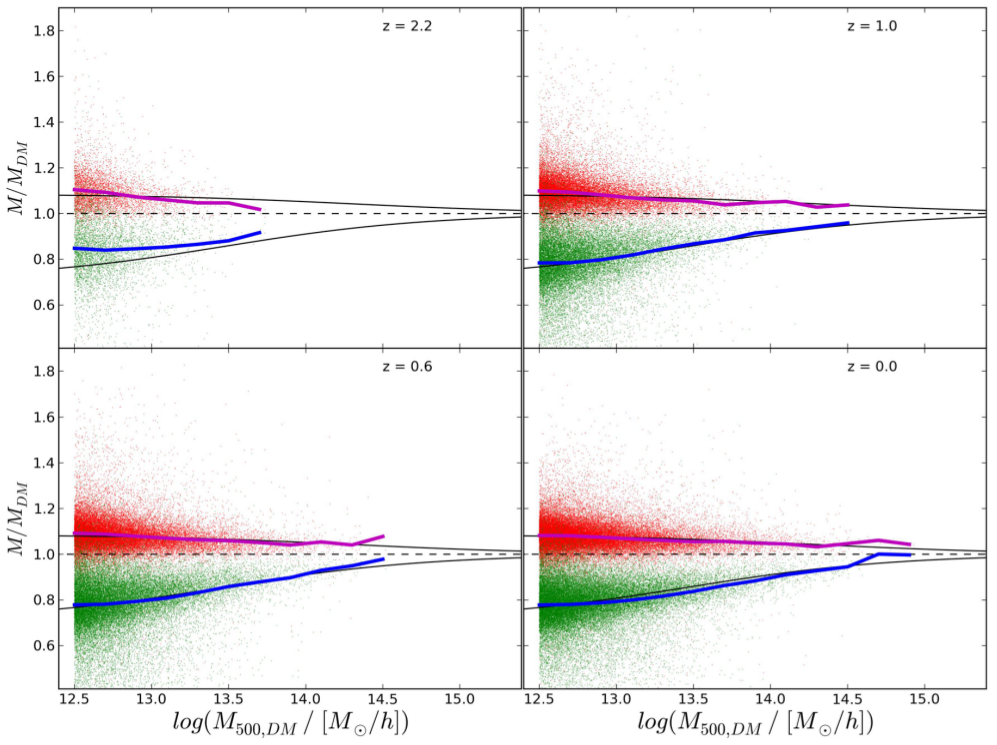
\includegraphics[width=0.7\textwidth]{Halo-mass-diff-cui2014}
  %   \vspace{-0.4cm}
  %   \caption{halo mass ($M_{500}$) difference respected to the DM run. Ref: Cui et al. 2014}
  % \end{figure}}
  \only<1>{
  \begin{figure}
    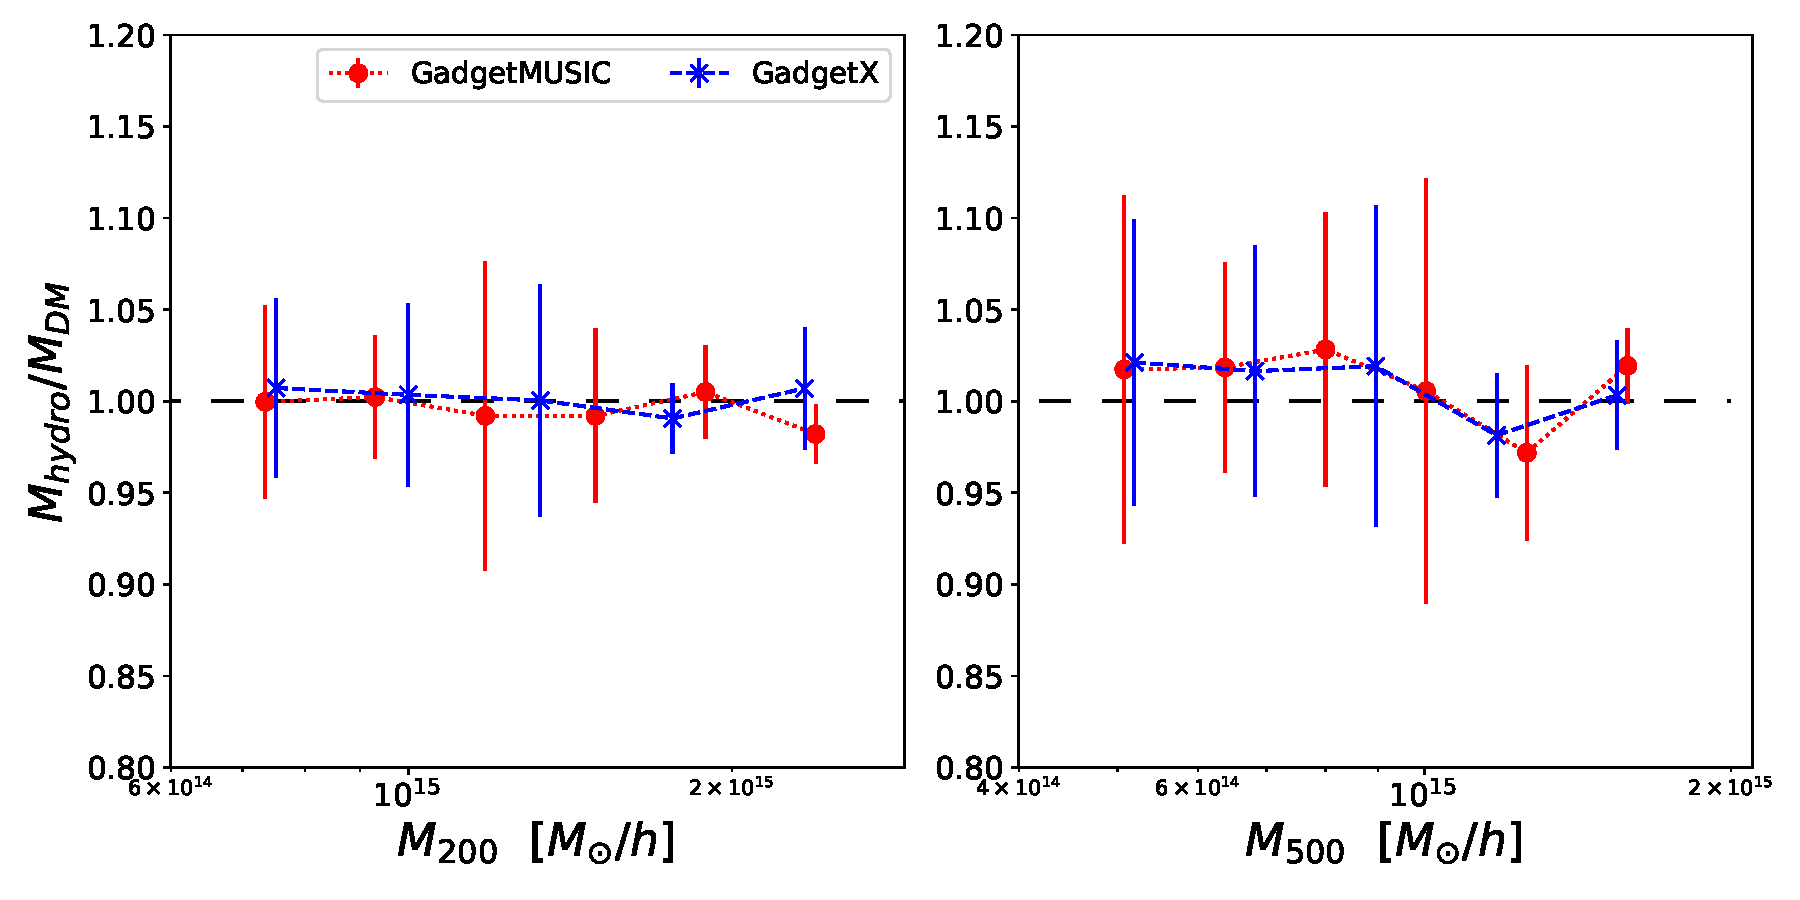
\includegraphics[width=\textwidth]{HMD.pdf}
    \vspace{-0.8cm}
    \caption{halo mass difference respected to the DM run. }
  \end{figure}}
  \only<2>{
  The mismatching problem.
  \begin{figure}
    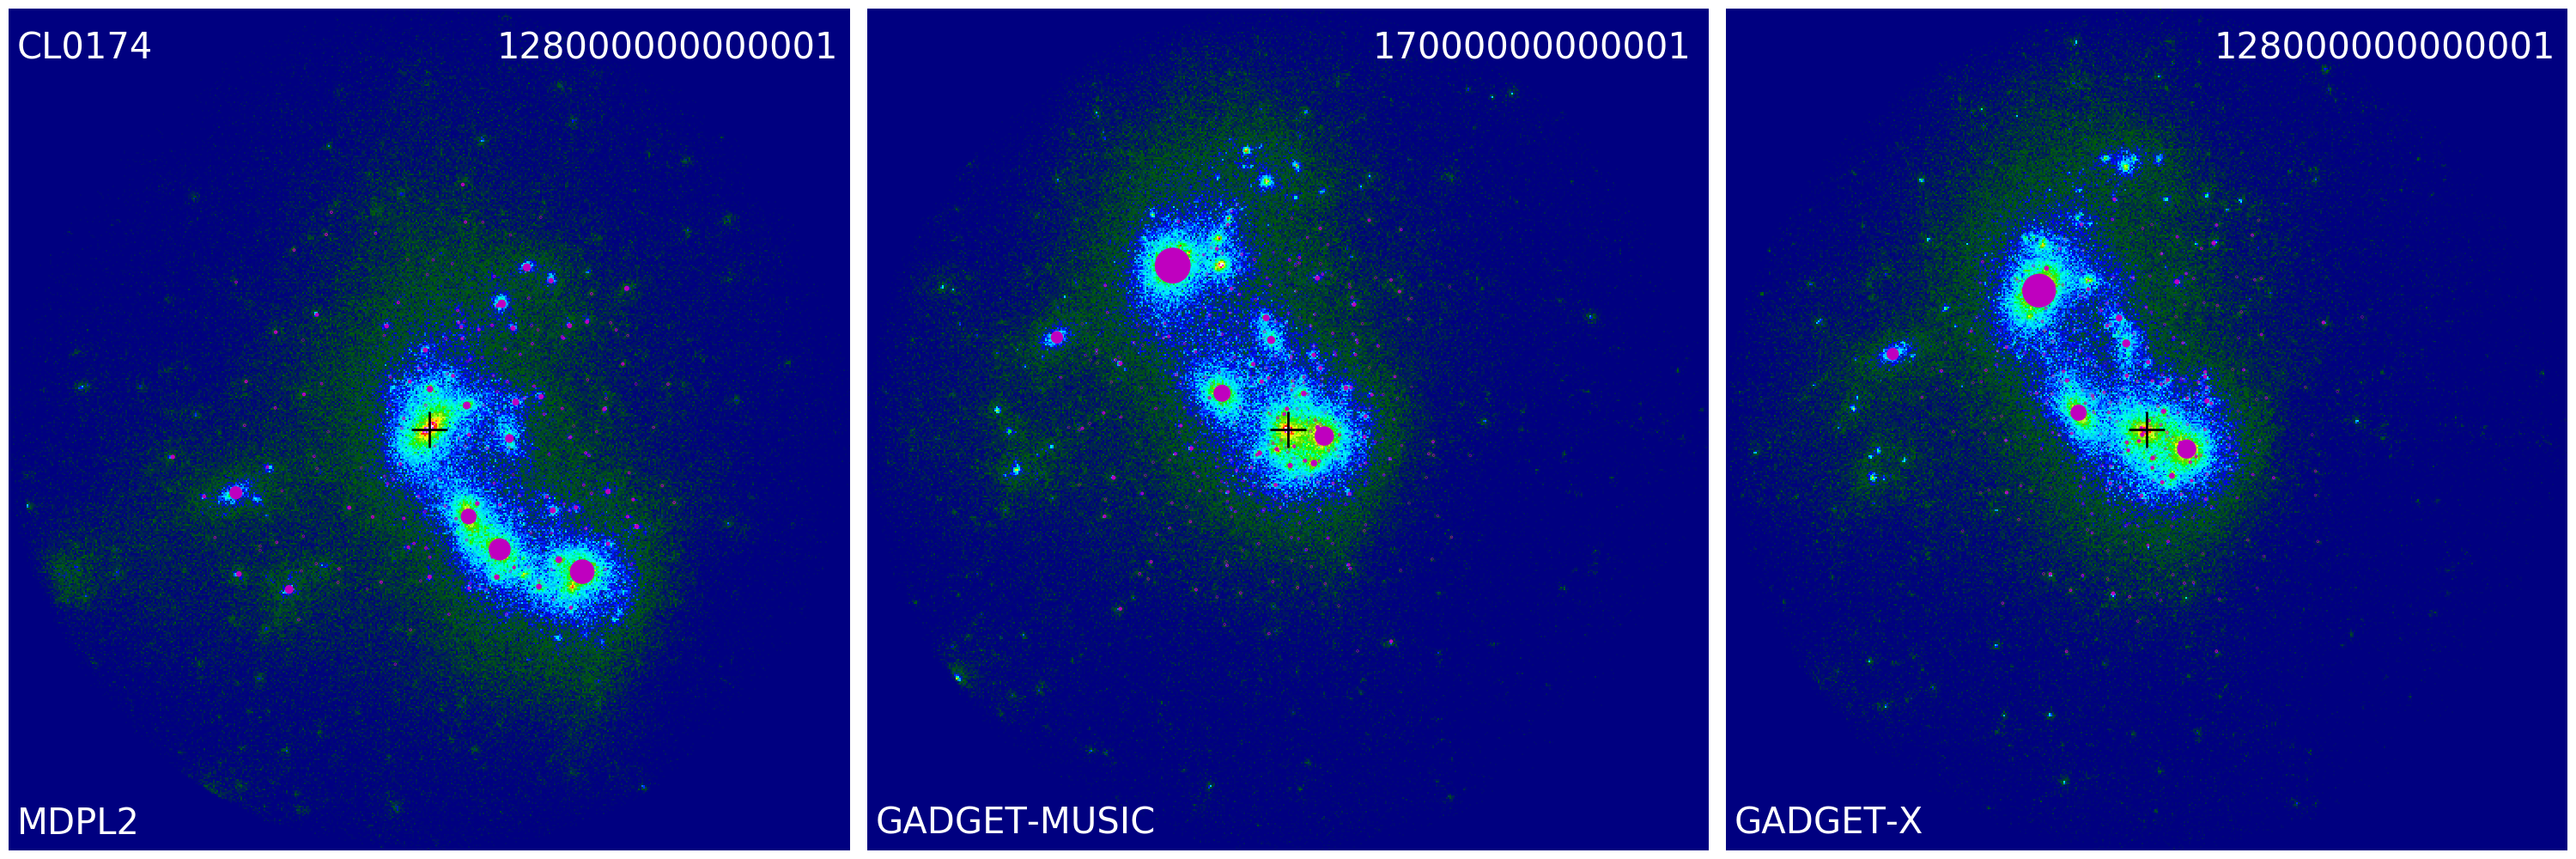
\includegraphics[width=\textwidth]{./plots/CL-0174_HID-01.png}
  \end{figure}
  Plots for the complete sample are available.
  }
\end{frame}

\begin{frame}
  \frametitle{General Properties: the dynamical state}
  We applied 3 criteria to classify the cluster's dynamical state to relaxed and un-relaxed: the virial ratio $\eta = (2T-E_s)/|W|$ with \alert{$0.85 < \eta < 1.15$}, center-of-mass offset $\Delta_r = |R_{cm} - R_{c}|/R_{200c} <$ \alert{0.04} and subhalo mass fraction $f_s = \sum M_{sub}/M_{200c} <$ \alert{0.1}.
  \only<1>{
    \begin{figure}
      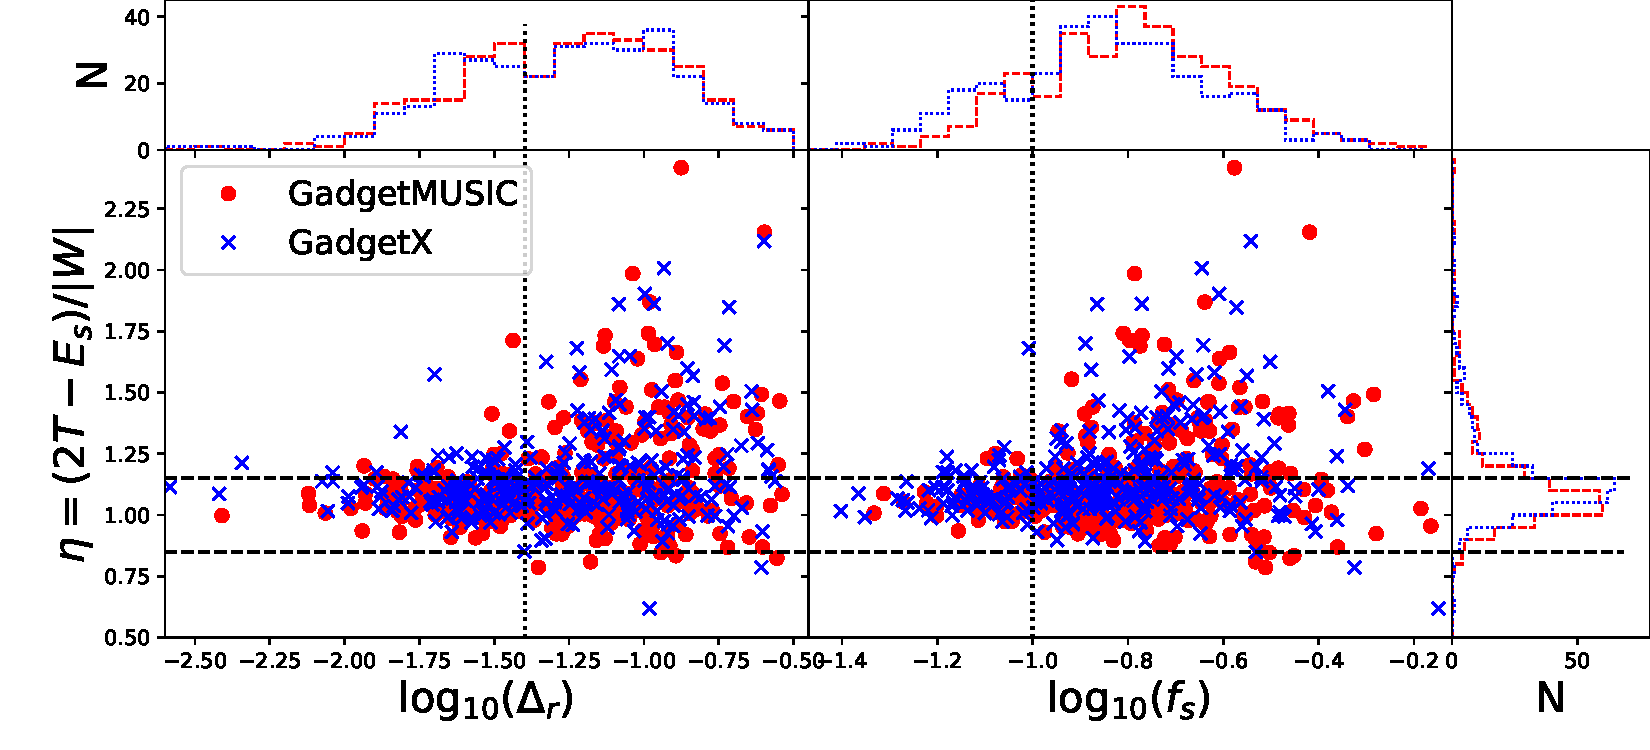
\includegraphics[width=0.9\textwidth]{ds-relations}
      \vspace{-0.4cm}
      \caption{The relations between the three parameters. }
    \end{figure}}
  \only<2>{
    \vspace{-0.8cm}
    \begin{columns}[t]
      \begin{column}{1.0\textwidth}
        \begin{table}
          \centering
          \caption{The fractions of relaxed clusters with different combinations of criteria.}
          \label{tab:relaxation}
          \begin{tabular}{lccc} % four columns, alignment for each
            \hline
            $M_{200c}$ & $\eta$, $\Delta_r$ \& $f_s$ & $\Delta_r$ \& $f_s$ & $f_s$ \\
            $10^{14} \hMsun$& MUSIC/X & MUSIC/X & MUSIC/X\\
            \hline
            $0.10 - 0.50$		& 0.44 / 0.36 & 0.56 / 0.48 & 0.70 / 0.65\\
            $0.50 - 1.00$		& 0.36 / 0.34 & 0.45 / 0.46 & 0.56 / 0.57\\
            $1.00 - 6.41$ 	& 0.27 / 0.29 & 0.30 / 0.35 & 0.43 / 0.48\\ \hdashline
            $6.41 - 10$   	& \alert{0.18 / 0.21} & 0.20 / 0.24 & 0.21 / 0.26\\
            $> 10 $ 		    & 0.06 / 0.08 & 0.07 / 0.13 & 0.07 / 0.14\\
            % \hline
          \end{tabular}
        \end{table}
      \end{column}
    \end{columns}
  }
\end{frame}

\begin{frame}
  \frametitle{General Properties: the CC fractions}
  Methods: Rossetti et al. 2001. Further, we verified that using the central entropy gives the same CC fraction.
\begin{columns}
  \begin{column}{\textwidth}
    \begin{table}
      \centering
      \caption{The Cool Core cluster fraction in the complete sample: $f_{CC} = \frac{N_{CC}}{N_{total}}$, the CC fraction in dynamically relaxed clusters $f_{CC/dr} = \frac{N_{CC, relaxed}}{N_{relaxed}}$ and the relaxation fraction in CC $f_{dr/CC} = \frac{N_{CC, relaxed}}{N_{CC}}$.}
      \label{tab:ccf}
      \begin{tabular}{lccc} % four columns, alignment for each
        \hline
        Simulation & $f_{CC}$ & $f_{CC/dr}$ & $f_{dr/CC}$ \\
        \hline
        {\sc MUSIC}	& \alert{0.09} & 0.04 & 0.07\\
        {\sc X} 		& \alert{0.26} & 0.33 & 0.21\\
        % \hline
      \end{tabular}
    \end{table}
  \end{column}
\end{columns}
\end{frame}

\begin{frame}
  \frametitle{General Properties: the baryon fractions}
  \only<1>{
  \begin{figure}
    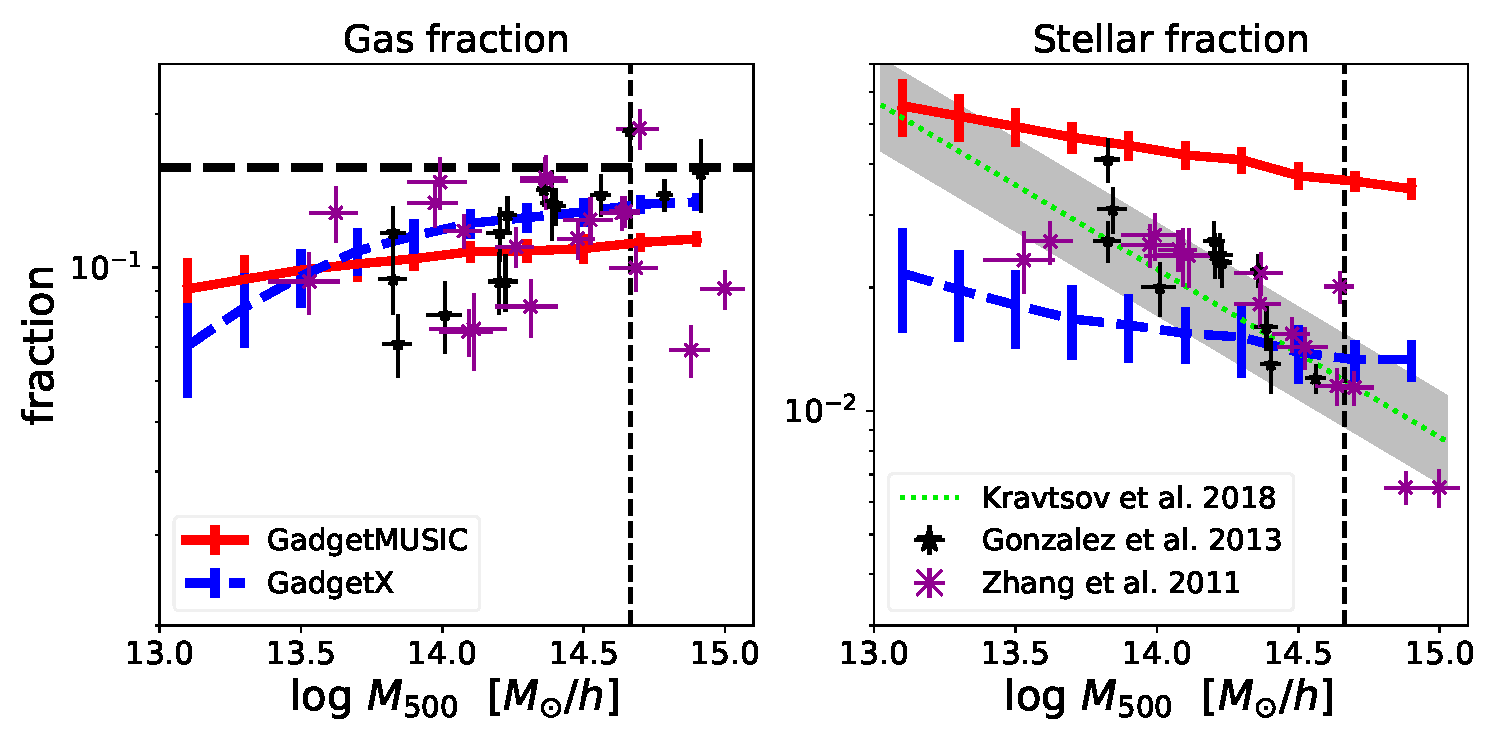
\includegraphics[width=\linewidth]{Baryonic-fractions-hydro-full}
    \vspace{-0.8cm}
    \caption{The baryon fractions compared with observations.}
  \end{figure}}
  \only<2>{
  \begin{figure}
    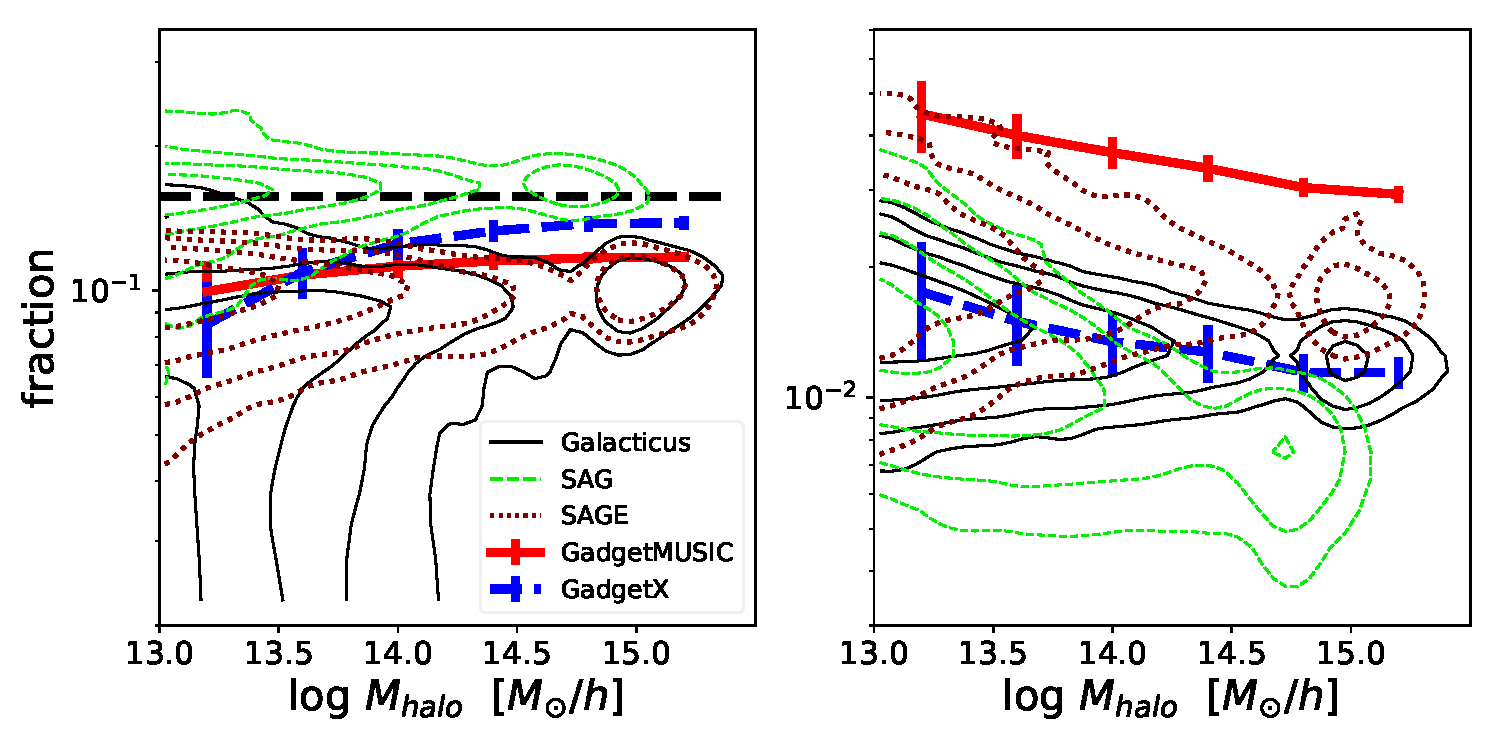
\includegraphics[width=\linewidth]{Baryonic-fractions-semi-full}
    \caption{The baryon fractions in halo compared with SAMs.}
  \end{figure}}
\end{frame}

\subsection{Scaling relations}
\begin{frame}
  \frametitle{Optical relations}
  The complete sample is used here.
  \begin{figure}
    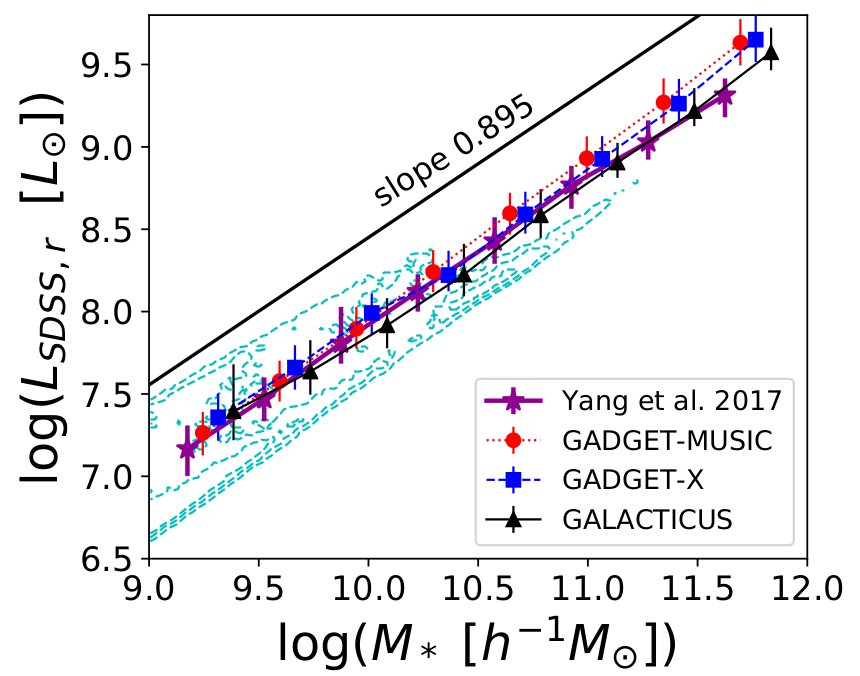
\includegraphics[width=0.4\linewidth]{./plots/Optical-relation1}
    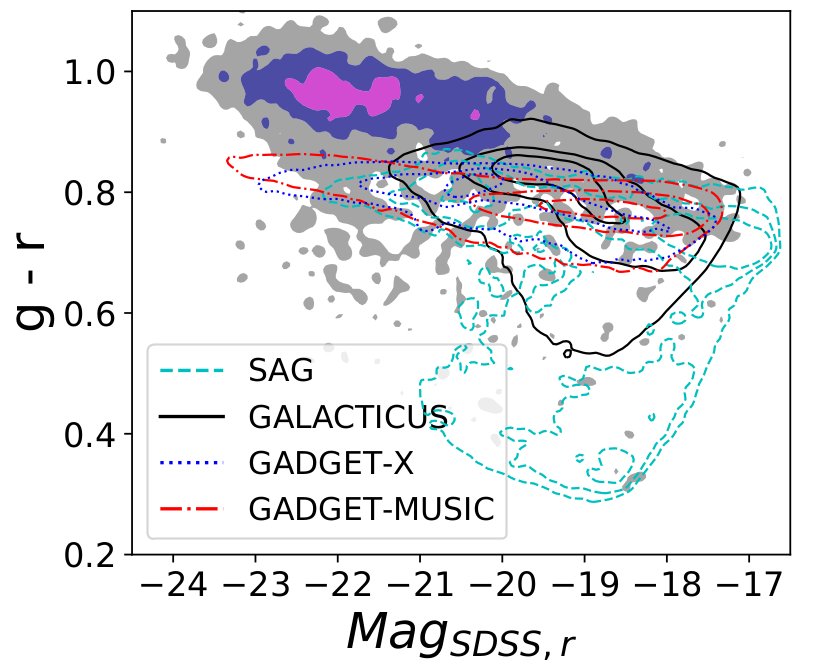
\includegraphics[width=0.385\linewidth]{./plots/Optical-relation2}
    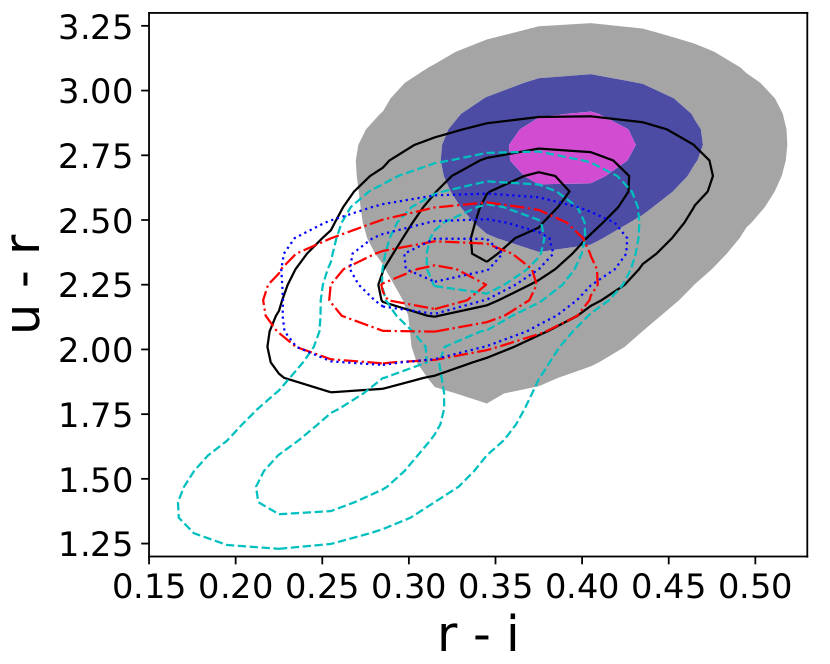
\includegraphics[width=0.38\linewidth]{./plots/Optical-relation3}
  \end{figure}
\end{frame}
\begin{frame}
  \frametitle{Optical relations: the satellite stellar mass function}
  The complete sample is used here.
  \begin{figure}
    \includegraphics<1>[width=0.8\linewidth]{Ssmf}
  \end{figure}
\end{frame}
\begin{frame}
  \frametitle{Optical relations: the stellar mass -- halo mass relation}
  The full sample is used here.
  \begin{figure}
    \includegraphics<1>[width=0.8\linewidth]{HS-relation-full}
  \end{figure}
\end{frame}
\begin{frame}
  \frametitle{Gas scaling relations}
  \begin{figure}
    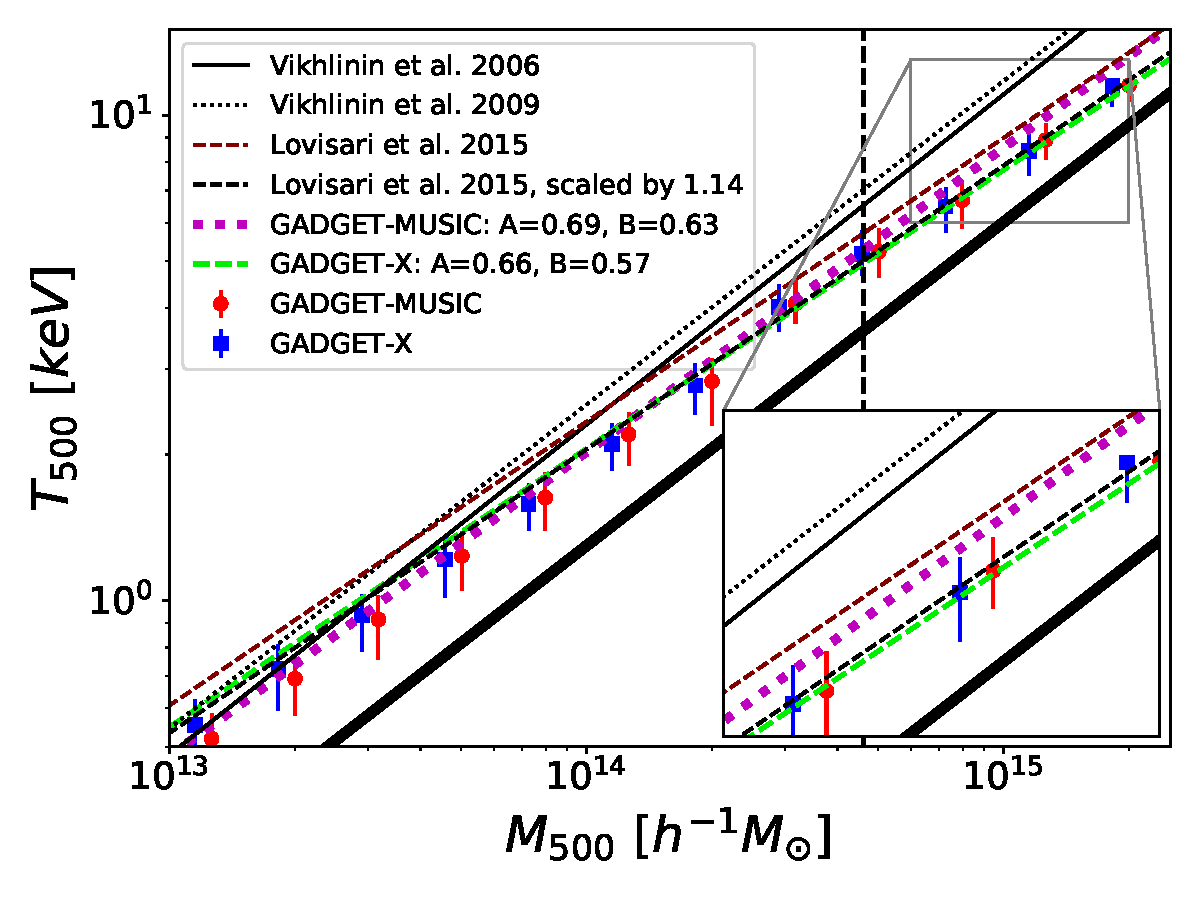
\includegraphics[width=0.49\linewidth]{T-M-relations}
    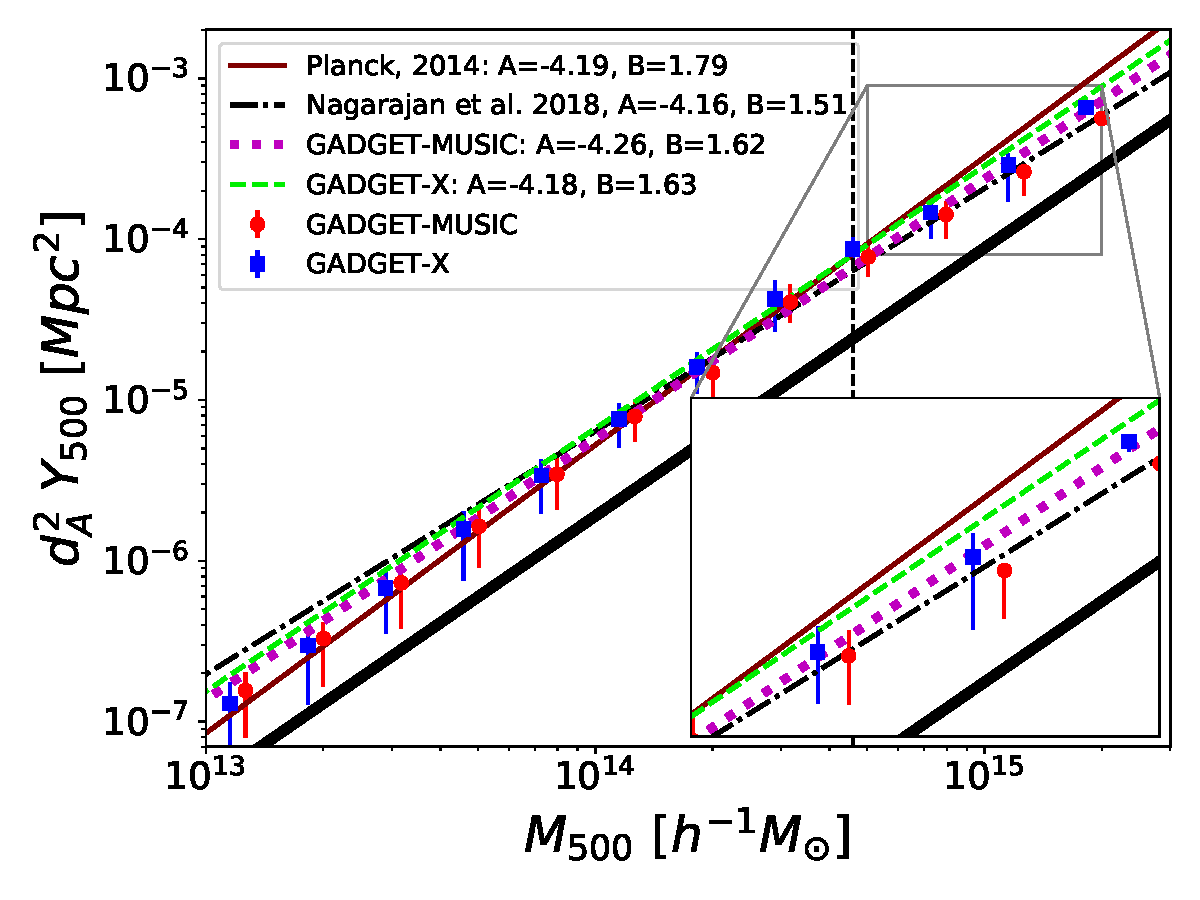
\includegraphics[width=0.49\linewidth]{YM_relation-full}
    \vspace{-0.4cm}
    \caption{The T-M (left) and Y-M (right) gas relations. }
  \end{figure}
\end{frame}

\section{conclusion and future prospects}
\begin{frame}
  \frametitle{Conclusion}
  {
  \begin{itemize}
    \item The baryons have a negligible impact on $M_{200}$, but increase $M_{500}$ for both hydro-simulations.
    \item $\sim 20 \%$ of the complete sample is relaxed clusters, 26\% (9\%) of the sample is CC for GadgetX (MUSIC).
    \item The baryon fractions are in agreement with the observations at massive halo masses for GadgetX.
    \item The optical relations are in agreement with the observations but the galaxies from more models seem to be a little blue. The BCG+ICL is a little bit too massive.
    \item The gas relations are generally in agreement with observations.
  \end{itemize}}
\end{frame}

% \begin{frame}
%   \frametitle{Future works}
%   \begin{itemize}
%     \item The density profiles, Mostoghiu et al. in prep.
%     \item The environment effects, Wang et al. in prep.
%     % \item Comparisons between different methods for estimating cluster dynamical states.
%     \item The mock images in optical, X-ray and SZ (lower images). \alert{And more...}
%       \begin{figure}
%         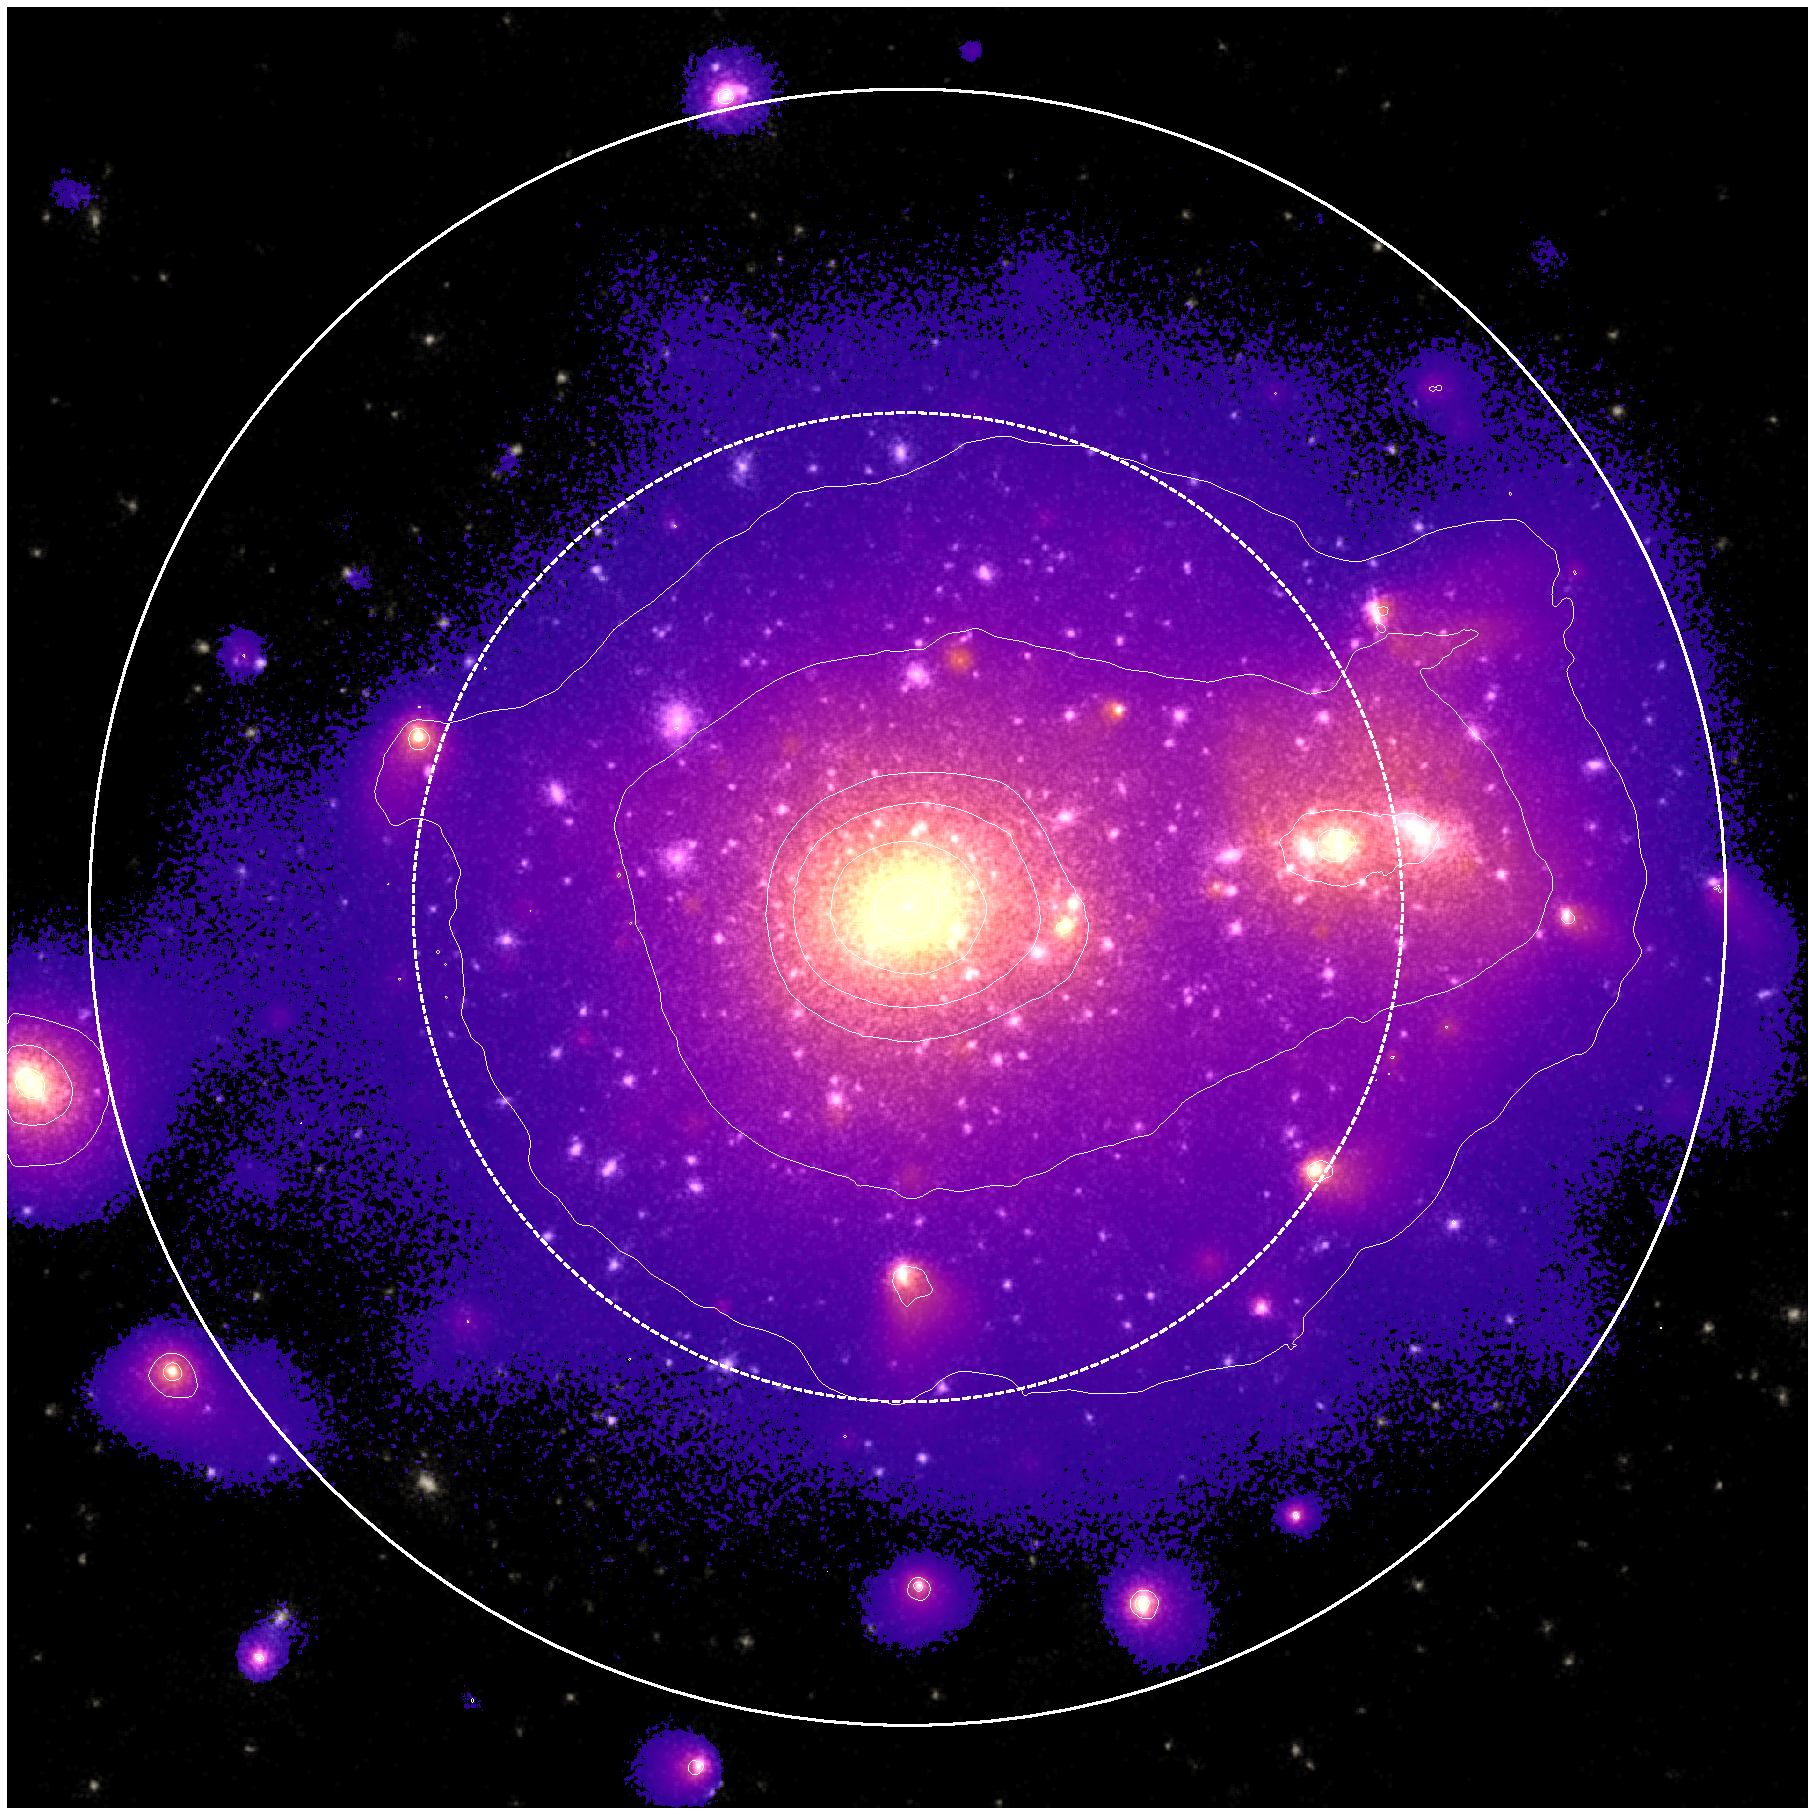
\includegraphics[width=0.48\linewidth]{./plots/Music-17-image}
%         \includegraphics[width=0.48\linewidth]{./plots/G3X-17-image}
%       \end{figure}
%   \end{itemize}
% \end{frame}
\end{document}
